\documentclass[12pt]{scrartcl}
\usepackage[margin=1in]{geometry}
\usepackage{hyperref}
\usepackage[T1]{fontenc}
\usepackage[utf8]{inputenc}
\usepackage[ngerman]{babel}
\usepackage{graphicx}
\usepackage{amsmath}
\usepackage{framed,enumitem}


\begin{document}
    \title{Project}
    \author{Fabian Otto -- Matrikelnummer: 2792549\\
    Foundations of Language Technology}
    \maketitle

    \section{Datenstruktur}

    Die Aufgabe ist es eine Sentimentanalyse für den IMDB Corpus auszuführen.
    Hierfür stehen jeweils 12.500 Reviews für das negative und positive Sentiment zur Verfügung.
    Zusätzlich werden auch noch weitere Datensätze angeboten, die ohne Labels sind.
    In diesem Projekt wurde diese Datenquelle jedoch nicht herangezogen.
    Die Reviews weisen ca. ein Länge von 500 bis 2.500 Zeichen auf und bieten damit eine ausreichende Länge, um Features zu extrahieren und die Stimmung des Verfassers zu identifizieren.
    Ein beispielhafter Datensatz sieht folgendermaßen aus:
    \begin{quote}
        \textit{
        Bromwell High is a cartoon comedy.
        It ran at the same time as some other programs about school life, such as "Teachers".
        My 35 years in the teaching profession lead me to believe that Bromwell High's satire is much closer to reality than is "Teachers".
        The scramble to survive financially, the insightful students who can see right through their pathetic teachers' pomp,
        the pettiness of the whole situation, all remind me of the schools I knew and their students.
        When I saw the episode in which a student repeatedly tried to burn down the school, I immediately recalled ......... at .......... High.
        A classic line: INSPECTOR: I'm here to sack one of your teachers.
        STUDENT: Welcome to Bromwell High.
        I expect that many adults of my age think that Bromwell High is far fetched.
        What a pity that it isn't!
        }
    \end{quote}

    Für die untenstehenden Ansätze wird immer das Vorgehen während der Dev Phase beschrieben.
    Gleiches gilt auch für die gezeigten Confusion Matrizen, die Evaluationskennzahlen befinden sich in der Readme.md.
    Zudem sind alle Train:Dev splits auf 80:20 gesetzt worden.
    Die Ergebnisse für die Testdaten finden sich in Codalab.

    \section{Naïve Bayes Ansatz}\label{sec:naiveBayesApproach}
    Mein erster Versuch basiert auf dem Ansatz der vorherigen Hausübung.
    Er extrahiert manuell Features, um im Anschluss einen Naïve Bayes einzusetzen, der das Sentiment bestimmt.

    Bezüglich der Features werden dabei vor allem die Wörter selbst als auch Bigramme herangezogen.
    Dies trägt dazu bei, wenn Wörter verstärkt in einer der Klassen ausgeprägt sind, dass diese Klasse wahrscheinlicher als Vorhersage wird.
    Weiterhin werden Uni-/Bigramm Scores ermittelt.
    Diese basieren auf der Anzahl der häufigsten Uni-/Bigramme im Trainingscorpus.
    Dies stellt letztendlich eine Gewichtung der obigen beiden Features mit der Frequenz im Trainingscorpus dar.
    Allerdings trägt die Verwendung dieses Features nicht so stark, wie erwartet, zu den Ergebnissen bei.
    Vor allem da Wörter (auch nach Stopwort Bereinigung) in beiden Klassen ähnlich häufig sind (z.B.\glqq{}gut\grqq{}).
    Auch die Suche nach Schimpfwörter brachte keine wesentliche verbesserung für diesen Corpus.
    Allerdings konnten mit einer Accuracy von 0.891 durchaus gut Ergebnisse erzielt werden.

    \section{TfIdf Ansatz}\label{sec:tfidfAnsatz}
    Eine zweite Herangehensweise an das Problem basiert auf der Ermittlung des TfIdf Vectors für die jeweiligen Reviews.
    TfIdf verfolgt die Idee, dass für jedes Wort $w$ die Frequenz innerhalb des Dokuments $d$ bzw., in dem vorliegenden Problem, der Review.
    Zudem wird durch die Berechnung der Dokumentenfrequenz, d.h. wie viele Dokumente $d$ im Corpus $w$ beinhalten, verhindert,
    dass insgesamt sehr frequente Wörter (the, a, etc.) zu stark gewichtet werden.
    Die konkrete Ausprägung, die im Rahmen von Sklearn hier eingesetzt wird, setzt sich wie folgt zusammen:

    \begin{equation}
        w_{t,d} = \left(1 + \log\left(tf_{t,d}\right)\right) \cdot \log\left(\frac{1 + N}{1 + df_{t}} + 1\right)
    \end{equation}

    Zudem wird eine Kosinus-Normalisierung vorgenommen.
    Von Sklearn wird hierfür ein Pipeline-Ansatz zur Verfügung gestellt,
    der sowohl einen CountVector erstellt als auch im Anschluss die TfIdf Scores berechnet.
    Am Ende wird ein Classifier bereitgestellt, der anhand der TfIdf Vectoren die Klassen bestimmt.
    Hierbei sind zum Vergleich Multinominal Naïve Bayes (MNB) und Stochastic Gradient Descent (SGD) verwendet worden.
    Letzteres ist laut der Webseite von Sklearn bereits oft erfolgreich in NLP Problemen eingesetzt worden.\footnote{\url{http://scikit-learn.org/stable/modules/sgd.html}}
    Dabei ergeben sich folgende Ergebnisse:

    \begin{figure}[h]
    	\begin{minipage}{0.45\textwidth}
    		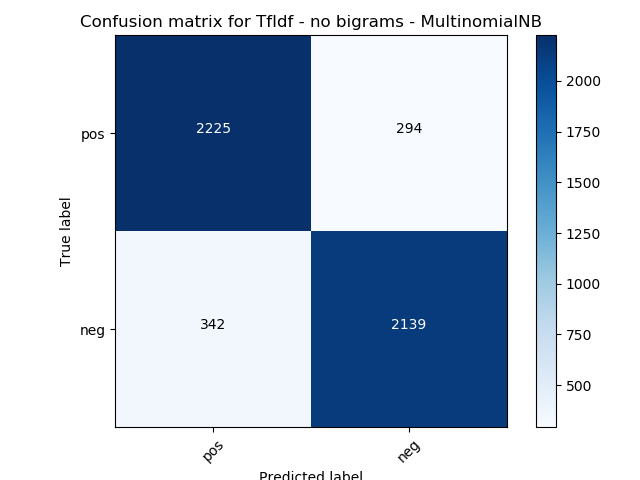
\includegraphics[scale=.35]{pictures/tfidf_nb_mnb.png}
    	\end{minipage}
    	\hfill
    	\begin{minipage}{0.45\textwidth}
    		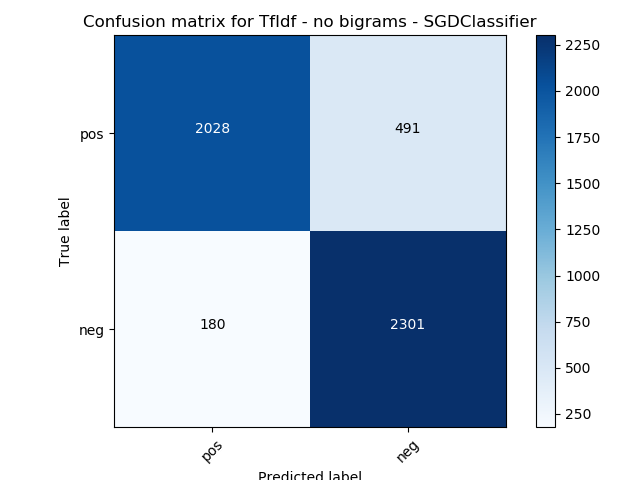
\includegraphics[scale=.35]{pictures/tfidf_nb_sgd.png}
    	\end{minipage}
    	\caption{Confusion Matrix für Multinomial Naïve Bayes und Stochastic Gradient Descent.}
    \end{figure}

    Zusätzlich besteht die Möglichkeit $n$-gramme Ranges einzusetzten.
    Dabei ergibt sich folgenden Ergebnis für $n \in \{1,\dots, 3\}$

        \begin{figure}[h]
    	\begin{minipage}{0.45\textwidth}
    		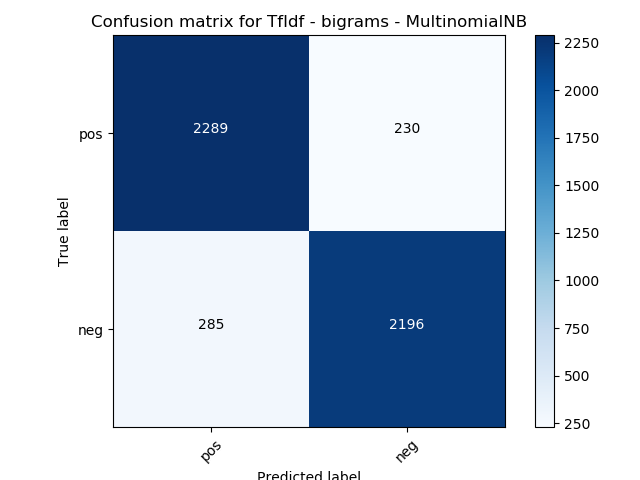
\includegraphics[scale=.35]{pictures/tfidf_b_mnb.png}
    	\end{minipage}
    	\hfill
    	\begin{minipage}{0.45\textwidth}
    		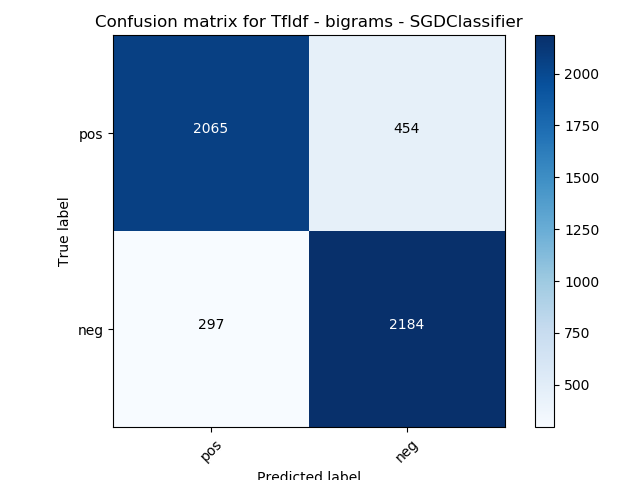
\includegraphics[scale=.35]{pictures/tfidf_b_sgd.png}
    	\end{minipage}
    	\caption{Confusion Matrix für Multinomial Naïve Bayes und Stochastic Gradient Descent mit $n$-grammen.}
    \end{figure}

    Ohne Bigramme zeigt MNB eine bessere Bestimmung von positiven Reviews auf, wohingegen SGD für negative Reviews besser zu funktionieren scheint.
    Beim Einsatz von Bigrammen zeigen die Ergebnisse ein leichte Verbesserung mit MNB im Vergleich zu SGD .
    Wobei insgesamt bei MNB mit Bigrammen die besten Resultate zu finden sind mit einem F-Score von knapp unter 90\%.

    \section{Paragraph Word Vectors}\label{sec:paragraphWordVectors}


\end{document}

